
\documentclass[a4paper,12pt]{scrbook}
\usepackage{amsmath,amssymb,amsthm}
\usepackage{fancyvrb}
\usepackage{parskip}
\usepackage{lastpage}
\usepackage{verbatim,boxedminipage,enumitem}
\usepackage{ifthen}
\usepackage{color,graphicx}
\usepackage{pgf}
\usepackage{longtable}
\usepackage{upquote}
%\usepackage[all]{xy}
\usepackage{tobiShell}
\usepackage{tikz}
\usetikzlibrary{automata}
\usetikzlibrary{arrows}
\usepackage{pgf,pgfarrows,pgfnodes}
\usepackage{pgfplots}
\usepackage{circuitikz}
\usetikzlibrary{circuits}
\usetikzlibrary{circuits.logic.US}
\usepackage{mymath}
\usepackage{python}
%------------------------------------------------------------------
% Verbatim for console window - single line frame, no line numbers
%------------------------------------------------------------------
\DefineVerbatimEnvironment%
 {console}{Verbatim}
 {frame=single}

%--------------------------------------------------------
% Remove the vertical spacing before and after Verbatim.
%--------------------------------------------------------
\usepackage{atbeginend}
\BeforeBegin{console}{\mbox{}\\ \begin{minipage}{\textwidth}\vspace{3pt}}
\AfterEnd{console}{\vspace{4pt} \end{minipage} \\ }

\begin{document}
\thispagestyle{empty}

\begin{center}
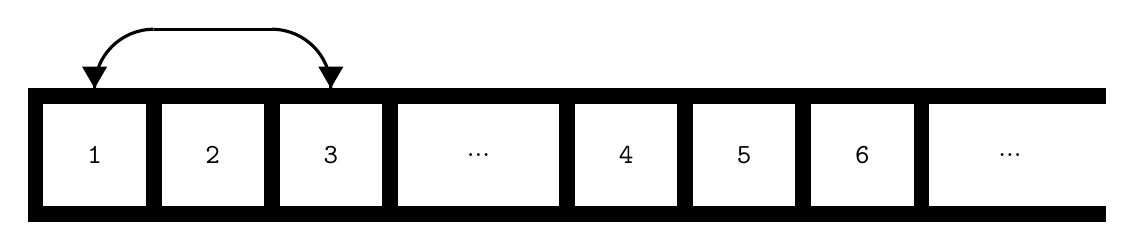
\begin{tikzpicture}

\draw (1.75, 1.75)
  node[draw, line width=0.2cm, , color=black,
       rounded corners=0cm, inner sep=0cm] {

\begin{minipage}[t][1.5cm]{1.5cm}
\mbox{}

\end{minipage}

};\draw (1.75, 1.75) node[color=black] {{\texttt{1}}};
\draw (3.25, 1.75)
  node[draw, line width=0.2cm, , color=black,
       rounded corners=0cm, inner sep=0cm] {

\begin{minipage}[t][1.5cm]{1.5cm}
\mbox{}

\end{minipage}

};\draw (3.25, 1.75) node[color=black] {{\texttt{2}}};
\draw (4.75, 1.75)
  node[draw, line width=0.2cm, , color=black,
       rounded corners=0cm, inner sep=0cm] {

\begin{minipage}[t][1.5cm]{1.5cm}
\mbox{}

\end{minipage}

};\draw (4.75, 1.75) node[color=black] {{\texttt{3}}};
\draw (6.625, 1.75)
  node[draw, line width=0.2cm, , color=black,
       rounded corners=0cm, inner sep=0cm] {

\begin{minipage}[t][1.5cm]{2.25cm}
\mbox{}

\end{minipage}

};\draw (6.625, 1.75) node[color=black] {...};
\draw (8.5, 1.75)
  node[draw, line width=0.2cm, , color=black,
       rounded corners=0cm, inner sep=0cm] {

\begin{minipage}[t][1.5cm]{1.5cm}
\mbox{}

\end{minipage}

};\draw (8.5, 1.75) node[color=black] {{\texttt{4}}};
\draw (10.0, 1.75)
  node[draw, line width=0.2cm, , color=black,
       rounded corners=0cm, inner sep=0cm] {

\begin{minipage}[t][1.5cm]{1.5cm}
\mbox{}

\end{minipage}

};\draw (10.0, 1.75) node[color=black] {{\texttt{5}}};
\draw (11.5, 1.75)
  node[draw, line width=0.2cm, , color=black,
       rounded corners=0cm, inner sep=0cm] {

\begin{minipage}[t][1.5cm]{1.5cm}
\mbox{}

\end{minipage}

};\draw (11.5, 1.75) node[color=black] {{\texttt{6}}};\draw[line width=0.2cm,black] (12.15,2.5) -- (14.6,2.5);
\draw[line width=0.2cm,black] (12.15,1.0) -- (14.6,1.0);
\draw (13.375, 1.75) node[color=black] {...};\draw[line width=0.04cm,black,->,>=triangle 60] (1.75,2.6001) -- (1.75,2.6);
\draw[line width=0.04cm,black,->,>=triangle 60] (4.75,2.6001) -- (4.75,2.6);
\draw[line width=0.04cm,black] (2.5,3.35) -- (4.0,3.35);
\draw[line width=0.04cm,black] (4.75,2.6001) arc (0:90:0.75);\draw[line width=0.04cm,black] (1.75,2.6001) arc (180:90:0.75);
\end{tikzpicture}

\end{center}

\end{document}
